	\documentclass[14pt]{extreport}
\usepackage{extsizes}
	\usepackage[frenchb]{babel}
	\usepackage[utf8]{inputenc}  
	\usepackage[T1]{fontenc}
	\usepackage{amssymb}
	\usepackage[mathscr]{euscript}
	\usepackage{stmaryrd}
	\usepackage{amsmath}
	\usepackage{tikz}
	\usepackage[all,cmtip]{xy}
	\usepackage{amsthm}
	\usepackage{varioref}
	\usepackage[ margin=1in]{geometry}
	\geometry{a4paper}
	\usepackage{lmodern}
	\usepackage{hyperref}
	\usepackage{array}
	\usepackage{float}
	\usepackage{easytable}
	 \usepackage{fancyhdr}\usepackage{longtable}
	 \usetikzlibrary{shapes.misc}
	 \newcommand\ang[1]{$#1{}^o$}
\newlength{\taillecellule}
\setlength{\taillecellule}{2cm}
\newcolumntype{C}{@{}>{\centering\arraybackslash}p{\taillecellule}@{}}

\renewcommand{\theenumi}{\alph{enumi})}
\usepackage{pstricks,multido}
\usepackage{arrayjob}
\usepackage{calc,xlop}
\tikzset{cross/.style={cross out, draw=black, minimum size=2*(#1-\pgflinewidth), inner sep=0pt, outer sep=0pt},
%default radius will be 1pt. 
cross/.default={1pt}}

	\pagestyle{fancy}
	\theoremstyle{plain}
	\fancyfoot[C]{\empty} 
	\fancyhead[L]{Contrôle bilan}
	\fancyhead[R]{22 avril 2024}
	
	
	
	\title{Contrôle de rentrée}
	\date{}
	\begin{document}



\subsection*{Exercice 1 : Calculs}  % 4 points
Recopiez et effectuez les calculs suivants : 

\begin{enumerate}
\item $2+3\times4\div2$
\item $5 - 2 + 3$
\item $ 3+2\times 4$
\item $ 5 + (-3) + 7 +  4 +  (-2) $
\item $ 3 - (-3) + 4 - 5 - (-2) + (-8)$
\item $(5-(-2) + 4) - (3- 2 + (-4))$
\end{enumerate}

\subsection*{Exercice 2 : Comparaisons}

Réduisez les fractions suivantes au même dénominateur : $\frac23$, $\frac59$, $\frac56$, $\frac{11}{18}$. 

Classez dans l'ordre croissant les nombres suivants : 

\[ \frac23; \ \  -\frac56;\ \   -0,5 ;\ \   1 ;\ \   \frac59 ;\ \   -\frac{11}{18}.\]

\subsection*{Exercice 3}

Parmi les données suivantes, lesquelles permettent de tracer un triangle ? Justifiez vos réponses. 

\begin{enumerate}
\item $AB = 3$ cm, $BC = 2$ cm, $AC = 6$ cm. 
\item $\widehat{ABC} =$ \ang{40}, $\widehat{BCA} =$ \ang{90}, $\widehat{CAB} =$ \ang{50}.
\item $AB = 5$ cm, $BC = 3$ cm, $AC = 7$ cm.
\item $\widehat{ABC} =$ \ang{30}, $\widehat{BCA} =$ \ang{50}, $\widehat{CAB} =$ \ang{90}.
\end{enumerate}

\subsection*{Exercice 4 - Tracé}

Sur la figure suivante, tracez : 
\begin{enumerate}
\item la médiatrice de $[AB]$
\item la hauteur issue de $C$
\item le symétrique du triangle $ABC$ par rapport à $(AB)$
\item le symétrique du triangle $ABC$ par rapport à $B$.
\end{enumerate}
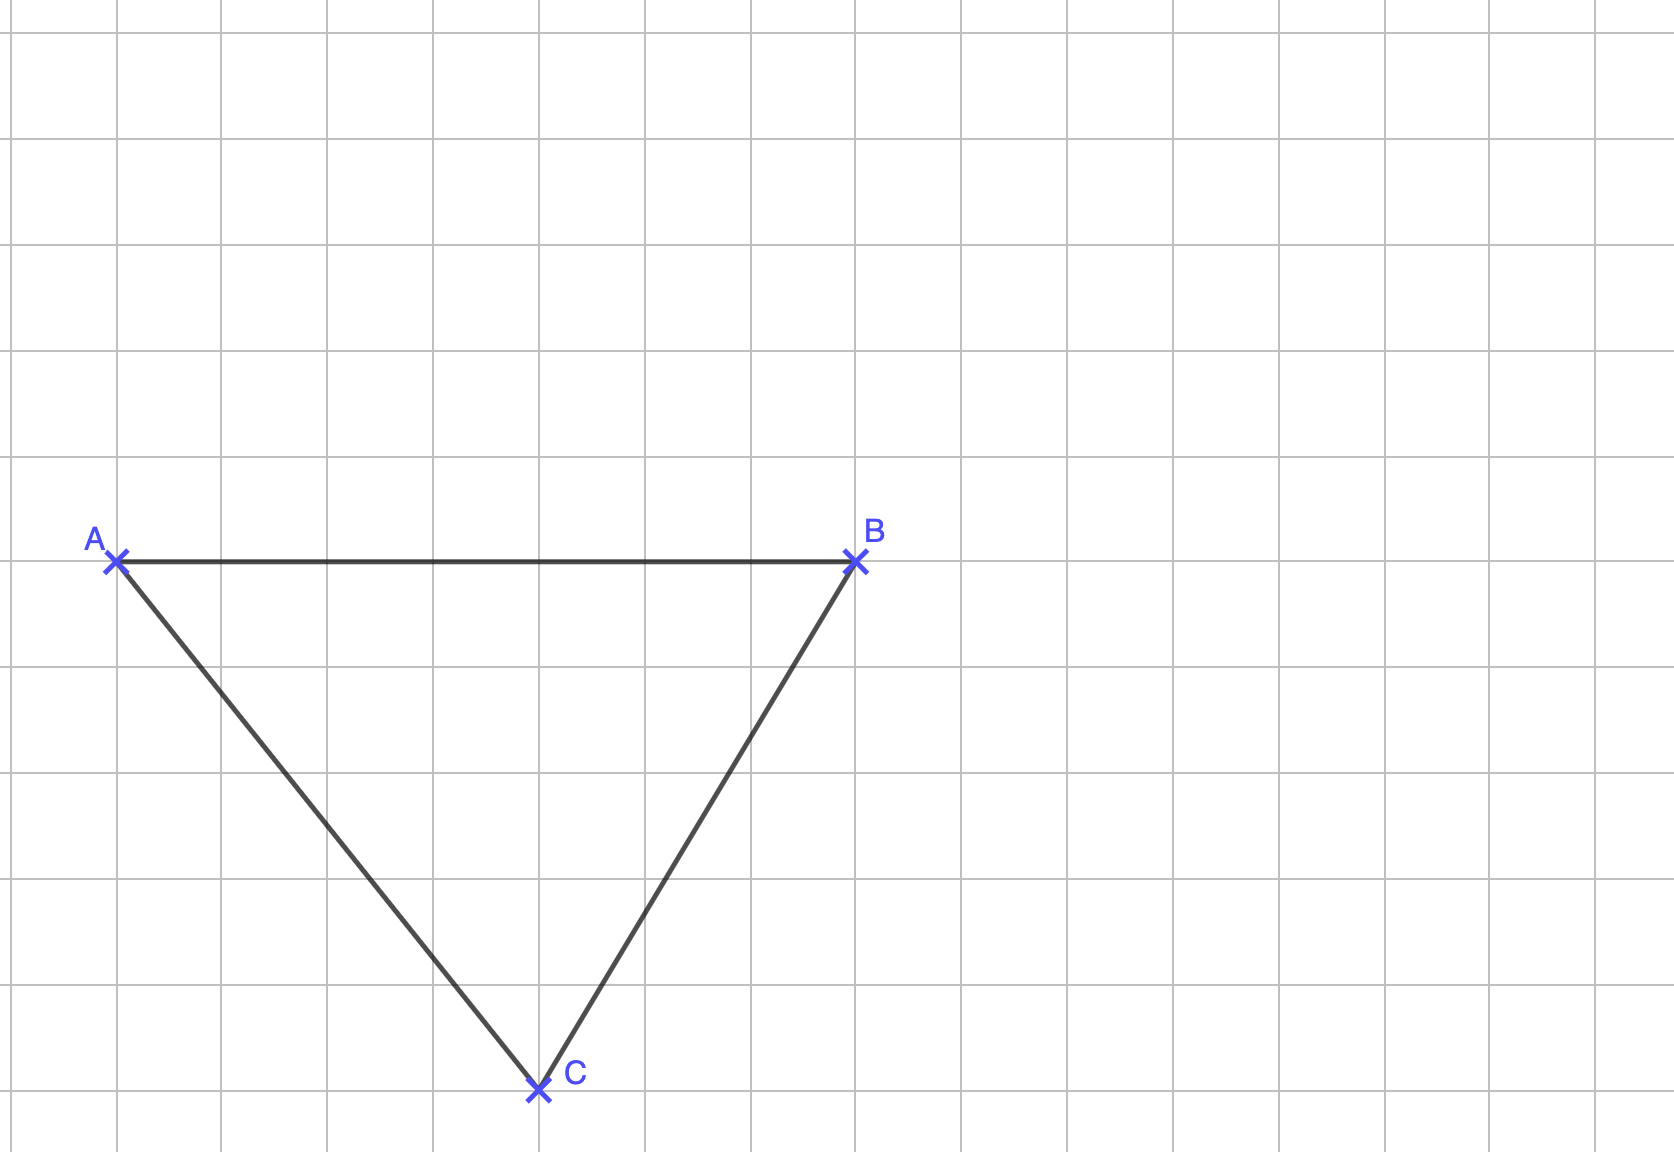
\includegraphics[scale=0.5]{Exos}
\subsection*{Exercice 5 - Angles}
	\begin{tikzpicture}[baseline]
    \tikzset{
      point/.style={thick, draw, cross out, inner sep=0pt, minimum width=5pt, minimum height=5pt,
      },
    }
    \clip (-1,-6.859954267158308) rectangle (9.893937016745921,3.298368333044762);
    	\draw[color={black}] (-49.337106354662005,-8.114802081529762)--(57.23104337140793,9.413170414574523);
	\draw[color={black}] (-43.01051039562473,25.49698162099757)--(50.800045009202414,-30.114681319318713);
	\draw[color={black}] (-32.54430446732648,-36.5053743530274)--(44.41902981165249,35.443898873669596);
	\draw[color={black}] (-49.10034384830023,-13.974751650033367)--(57.12663771366797,3.4970976845539177);
	\draw  [color={black},line width = 2,preaction={fill,color = {black},opacity = 0.2}] (0.9866000147758149,0.1631570570445111) -- (0,0) -- (0.8602101149709134,-0.5099395773234235) arc (-30.73:9.319999999999997:1) ;
	\draw [color={black}] (1.57,-0.3) node[anchor = center,scale=1, rotate = 0] {\ang{40}};
	\draw  [color={red},line width = 2,preaction={fill,color = {red},opacity = 0.2}] (4.841010222109848,-2.869763566876294) -- (3.980788327580091,-2.359843812402566) -- (4.711290183478223,-1.676933201590069) arc (42.82:-30.910000000000004:1) ;
	\draw [color={red}] (5.57,-2.19) node[anchor = center,scale=1, rotate = 0] {\ang{74}};
	\draw  [color={black},line width = 2,preaction={fill,color = {blue},opacity = 0.2}] (1.2237233194994683,-5.699013376196127) -- (0.23675925179005297,-5.859954267158308) -- (0.9672611725210718,-5.177043595736702) arc (42.82:9.009999999999998:1) ;
	\draw [color={black}] (1.67,-5.15) node[anchor = center,scale=1, rotate = 0] {\ang{34}}; 
	\draw [color={black}] (-0.5,0.5) node[anchor = center,scale=1, rotate = 0] {J};
	\draw [color={black}] (8.29,-4.62) node[anchor = center,scale=1, rotate = 0] {D};
	\draw [color={black}] (7.39,1.8) node[anchor = center,scale=1, rotate = 0] {W};
	\draw [color={black}] (3.98,-2.86) node[anchor = center,scale=1, rotate = 0] {U};
	\draw [color={black}] (0.74,-6.36) node[anchor = center,scale=1, rotate = 0] {I};

\end{tikzpicture}\\
\begin{enumerate}
\item  Déterminer la mesure de l'angle $\widehat{JUW}$. Justifiez.
\item  En déduire la mesure de l'angle $\widehat{UWJ}$.Justifiez.
\item  Déterminer si les droites $(JW)$ et $(ID)$ sont parallèles. Justifiez. \end{enumerate}
	
	
    
 
\end{document}